\section{Introduction}
\begin{figure}[t]
    \centering
    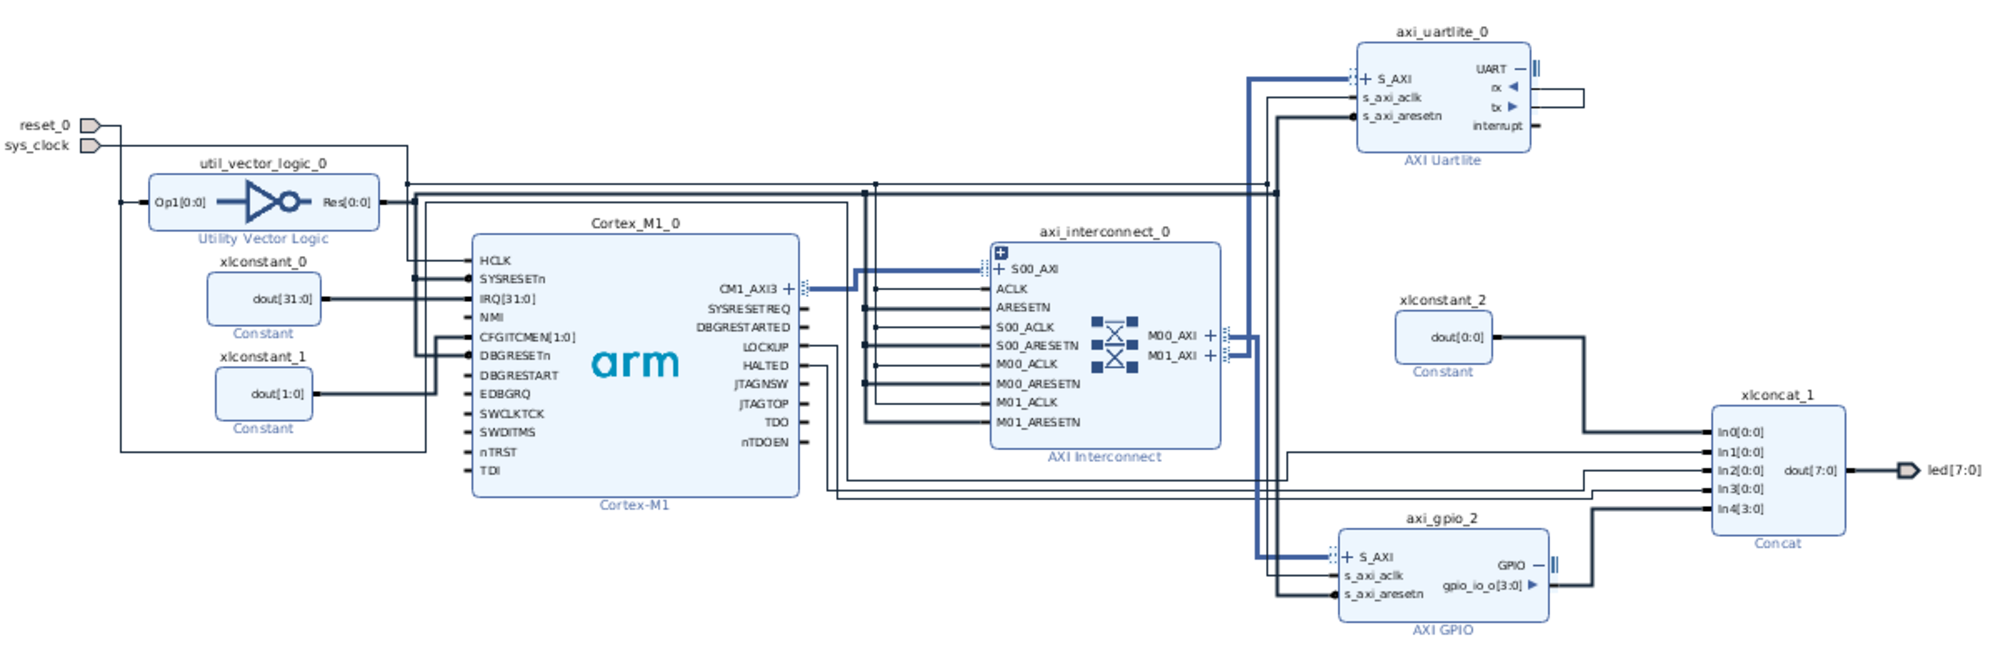
\includegraphics[width=\textwidth]{figures/pr_blockDesign.pdf}
    \caption{Block Diagram of the partial reconfiguration functionality}\label{fig:prBlockDesign}
\end{figure}

In this lab, fail-safe mechanisms for \glspl{ECU} are explored on the basis of \gls{PR} in \glspl{FPGA}.
The introduced design contains typical characteristics of an automotive system.
Communication of the different sub-systems is realized with a bus and connects the \gls{FPGA} to the \glspl{ECU} that handle operations during normal conditions. 
\glspl{ECU} are monitored by a bus monitor in the \gls{FPGA} for nominal operation characteristics and can be replaced by the instantiation of the very same \gls{ECU} within the \gls{FPGA} in case of failure.

Our \glspl{ECU} are based on the Cortex-M1, an ARM-based microcontroller that became recently available as an \gls{IP}-package for Xilinx based \glspl{FPGA}.
By using a common hardware base we were able to streamline the development of the control-software which enables a faster development process and reduces the overhead of functional verification.
 
Brief overview, problem statement and final outcome.

\subsection{Required Tools and packages}

\begin{itemize}
    \item Vivado 2018.3
    \item Vivado 2018.2
    \item uVision 5 (Windows only)
    \item ARM Keil (Windows only)
    \item ARM Cortex M1 IP for Vivado
\end{itemize}
